\newcommand{\svcourse}{CST Part IA: Software Engineering and Security}
\newcommand{\svnumber}{1}
\newcommand{\svvenue}{Microsoft Teams}
\newcommand{\svdate}{2022-05-11}
\newcommand{\svtime}{15:00}
\newcommand{\svuploadkey}{CBd13xmL7PC1zqhNIoLdTiYUBnxZhzRAtJxv/ytRdM1r7qIfwMsxeVwM/pPcIo8l}

\newcommand{\svrname}{Dr Sam Ainsworth}
\newcommand{\jkfside}{oneside}
\newcommand{\jkfhanded}{yes}

\newcommand{\studentname}{Harry Langford}
\newcommand{\studentemail}{hjel2@cam.ac.uk}


\documentclass[10pt,\jkfside,a4paper]{article}
\usepackage{graphicx}

% DO NOT add \usepackage commands here.  Place any custom commands
% into your SV work files.  Anything in the template directory is
% likely to be overwritten!

\usepackage{fancyhdr}

\usepackage{lastpage}       % ``n of m'' page numbering
\usepackage{lscape}         % Makes landscape easier

\usepackage{verbatim}       % Verbatim blocks
\usepackage{listings}       % Source code listings
\usepackage{graphicx}
\usepackage{float}
\usepackage{epsfig}         % Embed encapsulated postscript
\usepackage{array}          % Array environment
\usepackage{qrcode}         % QR codes
\usepackage{enumitem}       % Required by Tom Johnson's exam question header

\usepackage{hhline}         % Horizontal lines in tables
\usepackage{siunitx}        % Correct spacing of units
\usepackage{amsmath}        % American Mathematical Society
\usepackage{amssymb}        % Maths symbols
\usepackage{amsthm}         % Theorems

\usepackage{ifthen}         % Conditional processing in tex

\usepackage[top=3cm,
            bottom=3cm,
            inner=2cm,
            outer=5cm]{geometry}

% PDF metadata + URL formatting
\usepackage[
            pdfauthor={\studentname},
            pdftitle={\svcourse, SV \svnumber},
            pdfsubject={},
            pdfkeywords={9d2547b00aba40b58fa0378774f72ee6},
            pdfproducer={},
            pdfcreator={},
            hidelinks]{hyperref}

\renewcommand{\headrulewidth}{0.4pt}
\renewcommand{\footrulewidth}{0.4pt}
\fancyheadoffset[LO,LE,RO,RE]{0pt}
\fancyfootoffset[LO,LE,RO,RE]{0pt}
\pagestyle{fancy}
\fancyhead{}
\fancyhead[LO,RE]{{\bfseries \studentname}\\\studentemail}
\fancyhead[RO,LE]{{\bfseries \svcourse, SV~\svnumber}\\\svdate\ \svtime, \svvenue}
\fancyfoot{}
\fancyfoot[LO,RE]{For: \svrname}
\fancyfoot[RO,LE]{\today\hspace{1cm}\thepage\ / \pageref{LastPage}}
\fancyfoot[C]{\qrcode[height=0.8cm]{\svuploadkey}}
\setlength{\headheight}{22.55pt}


\ifthenelse{\equal{\jkfside}{oneside}}{

 \ifthenelse{\equal{\jkfhanded}{left}}{
  % 1. Left-handed marker, one-sided printing or e-marking, use oneside and...
  \evensidemargin=\oddsidemargin
  \oddsidemargin=73pt
  \setlength{\marginparwidth}{111pt}
  \setlength{\marginparsep}{-\marginparsep}
  \addtolength{\marginparsep}{-\textwidth}
  \addtolength{\marginparsep}{-\marginparwidth}
 }{
  % 2. Right-handed marker, one-sided printing or e-marking, use oneside.
  \setlength{\marginparwidth}{111pt}
 }

}{
 % 3. Alternating margins, two-sided printing, use twoside.
}


\setlength{\parindent}{0em}
\addtolength{\parskip}{1ex}

% Exam question headings, labels and sensible layout (courtesy of Tom Johnson)
\setlist{parsep=\parskip, listparindent=\parindent}
\newcommand{\examhead}[3]{\section{#1 Paper #2 Question #3}}
\newenvironment{examquestion}[3]{
\examhead{#1}{#2}{#3}\setlist[enumerate, 1]{label=(\alph*)}\setlist[enumerate, 2]{label=(\roman*)}
\marginpar{\href{https://www.cl.cam.ac.uk/teaching/exams/pastpapers/y#1p#2q#3.pdf}{\qrcode{https://www.cl.cam.ac.uk/teaching/exams/pastpapers/y#1p#2q#3.pdf}}}
\marginpar{\footnotesize \href{https://www.cl.cam.ac.uk/teaching/exams/pastpapers/y#1p#2q#3.pdf}{https://www.cl.cam.ac.uk/\\teaching/exams/pastpapers/\\y#1p#2q#3.pdf}}
}{}


\begin{document}

\begin{enumerate}[label=(\alph*)]

\item

\begin{enumerate}[label=(\roman*)]

\item Explain the collision detection mechanism applied in standard wired
medium access control associated with CSMA and indicate why this might be
unsuitable for wireless networks.

``Carrier Sense Multiple Access / Collision Detection'' (CSMA/CD) is the
standard wired medium access control. Senders listen on the link
to determine whether another node is transmitting on the link. The node
waits until the link is idle then transmits their message (Carrier Sense).

If any node detects a collision, they transmit a hash on the network to
inform other nodes of the collision. They continue to transmit this hash
until they no longer detect the collision. This means frames must be at
least $2 \cdot BDP$ such that the sending node is guaranteed to hear of the
collision \textit{before} they finish transmitting the packet (to avoid a
``late collision''). If the sender is alerted to a collision, they stop
transmission and perform a Binary Exponential Backoff before repeating the
process.

In Binary Exponential Backoff (BEB), the node starts with a small maximum
wait. When BEB is performed, a time is uniformly selected between 0 and the
maximum wait. Every time BEB is performed, the maximum wait is doubled.

This protocol struggles with wireless networks. In wireless, we experience
local collisions -- where one node hears a collision but others do not. So a
node may hear a collision and send a jamming signal, preventing all
transmission on the network when no node transmitting or receiving data
hears the collision.

In the example below, $N$ hears both $S_1$ and $S_2$; so transmits a jamming
signal telling both to stop transmitting due to a collision. However,
neither receivers $R_1$ or $R_2$ observe a collision. The critical
observation is that \textit{in wireless, collisions happen only at the
receivers}.
\begin{center}
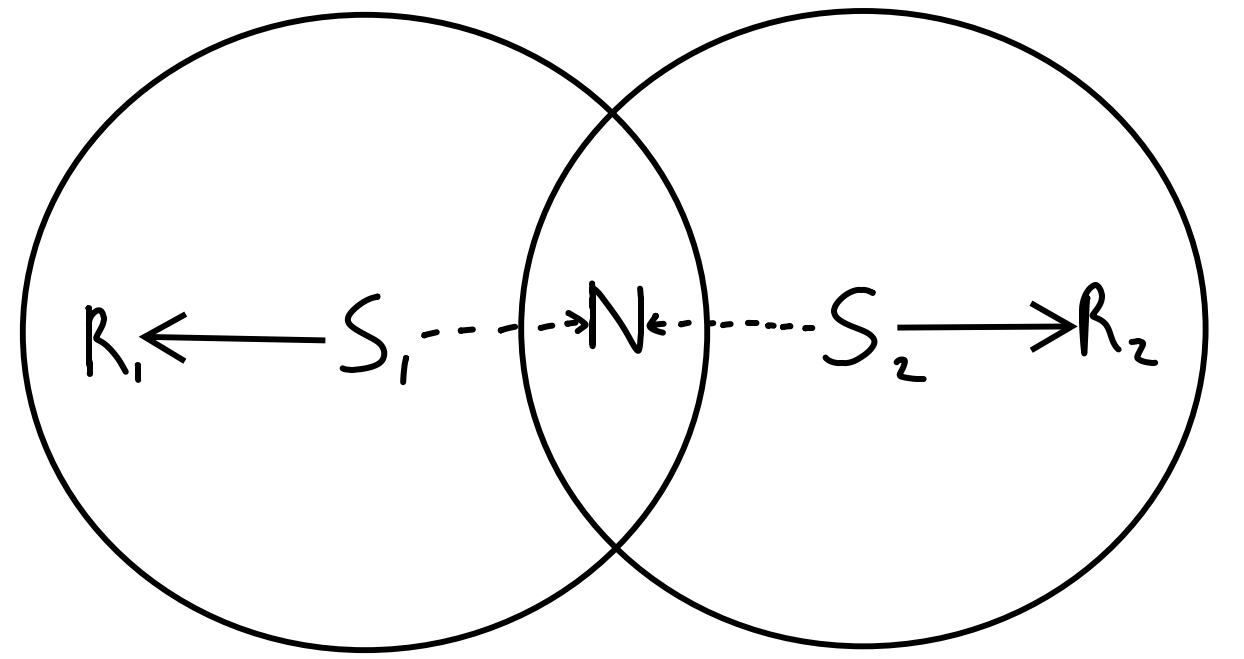
\includegraphics[width=0.6\textwidth]{csma_cd_failure}
\end{center}

Furthermore, many (older) devices cannot both listen and transmit on
wireless networks at the same time -- the signal they send
overwhelms their receiver.

\item Describe how CSMA/CA (Collision Avoidance) works and explain its
limitations.

In CSMA/CA if a node wants to send a message, it waits until the link is
idle using Carrier Sense. Once the link is idle, the node sends the data
and waits for a response. If the node doesn't receive a response, it
performs a Binary Exponential Backoff and repeats.

When using CSMA/CA, the sender must decide how long to wait for a response --
if it waits too long, it wastes time. If it's too short it sleeps and
unnecessarily retransmits messages.

CSMA/CA suffers from both the hidden and exposed terminal problems.
In wireless, signals suffer badly from attenuation and have a range.

In the hidden terminals problem; there may be two senders transmitting to
a receiver who can hear both -- but both senders are ouf of range of each
other so detect no issue. CSMA/CA solves this probabilistically using BEB
-- it wastes time and bandwidth.

In the exposed terminals problem; a node which wishes to send a message
hears a signal so does not transmit -- while the receiver is out of range
of the signal the sender hears; so it would be safe to send the message.

\item Illustrate how MACAW works and indicate its limitations on the
exposed terminal problem through an example.

\begin{itemize}

\item Nodes wishing to transmit data wait until it will not cause a
collision (more later) then send an RTS (request to send)

\item If a node hears a RTS for itself and responding would not cause a
collision, it responds with a CTS if it is able to safely receive the data.

\item Once the sender hears the CTS, it sends the data.

\item The receiver sends an acknowledgement ACK once it has received the data.

\item If a node hears a RTS for another node, then it is within transmission
range of a node which may shortly be receiving data. So it must wait until it
would have heard a CTS (using a timeout) before sending any data.

\item Once a node hears a CTS, it must defer transmission of data until it
hears the ACK\@.

\item Receivers which are in this state are \textit{unable} to respond with a
CTS since it would cause a collision.

So the sender would send an RTS then hear no CTS\@. This is addressed by the
use of an RRTS (request for request to send) -- ``I heard you wanted to send
data but couldn't respond then, lets try again now''.

\end{itemize}

In the exposed terminals problem, a node hears a CTS then a RTS\@. However,
since it heard a CTS, it's not safe for it to send its own CTS\@. This
wastes bandwidth, since it's \textit{safe} for the node wishing to send to
transmit.

\begin{center}
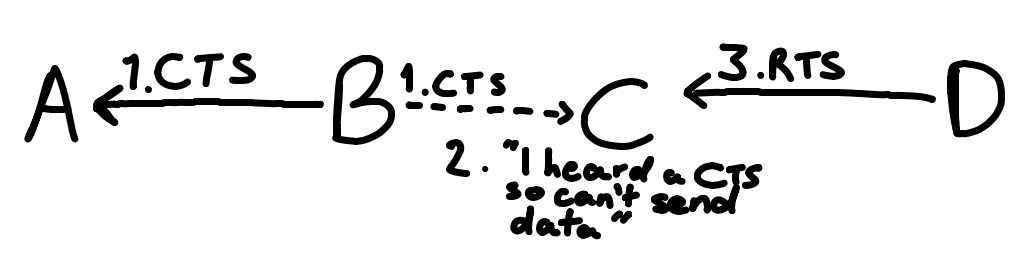
\includegraphics[width=0.8\textwidth]{macaw_diagram_png}
\end{center}

\item Would the deployment of MACAW be needed in an installation of a MAC
protocol for a single base station that communicates with some mobile
terminals? Why?

No; although it could be used for coordination in a more efficient protocol.
MACAW is designed to allow communication to happen concurrently between
many nodes over a shared wireless channel. In this system, there are many
channels and one node with which each mobile terminal wants to communicate
with. This provides an excellent opportunity for a coordinator-based
approach allowing mobile terminals to set up channels with the base station.
A MACAW-based approach would allow the base station to receive data from at
most one node at once -- such a system would be unusable (i.e only one
person in Cambridge can make a phone call at once).

A better solution would be to multiplex the channel into a number of smaller
channels (using FDMA and CDMA) coordinated by the base station. We still
have the problem of distributing frequencies and codes to mobile terminals
(setting up channels ). I propose having a single (or small set of) known
channels running the MACAW protocol on which requests to setup channels will
be made to the base station.

since the terminals are mobile, they can leave the network. We cannot
allocate channels permanently and must therefore have an expiry time for
each channel (ie $1h$) with a slightly higher expiry time on the base
station (ie $1.5h$) to account for possible clock drift.

However, there could exist ``zombie nodes'' whose clocks have a very high
drift. To resolve this, we \textit{could} run MACAW on each channel --
however since this is highly unlikely to occur and MACAW adds high latency
to data transmission. A better solution would be to use a modified version
of CSMA where sensors listen for $DIFS$ and setup a new channel if they
hear a node talking.

\end{enumerate}

\item

\begin{enumerate}[label=(\roman*)]

\item You are called upon, as expert, to design a wireless sensor network
to monitor environmental factors in a $500m^2$ area within a forest. Sensors
will record temperature every 30 minutes. Describe the requirements of the
network stack, considering how they differ from a traditional wired or
wireless Ethernet.

\begin{itemize}

\item The data throughput requirement is very low -- a double every 30 minutes.

\item The latency requirements are low -- we don't mind waiting a few seconds.

\item The sensors are wirelessly connected in a forest -- there are lots of
obstacles and conditions may vary wildly. This could cause a very high error
rates.

\item The sensor network must support broadcast -- sensors do not have
accurate timekeeping and so must be synchronised to ensure measurements are
taken at the same time.

\end{itemize}

\item Invent two different MAC layer protocols for sensor networks (perhaps
simplified versions of SMAC and XMAC) and then indicate which one you would
employ for your network and why.

I propose two protocols. The first uses Polling and the second uses a
Random Access Protocol. The first protocol has the lowest technology
requirements, while the second is built on existing technology.

\begin{itemize}

\item The first protocol takes advantage of the latency and bandwidth
requirements and uses polling.

Every 30 minutes, the coordinator broadcasts it's current time and asks all
the sensors to synchronise their clocks and record their current reading. The
coordinator then polls each of the sensors asking for their most recent
reading. Sensors also synchronise when they are polled.

If Sensors do not hear any synchronise broadcast, they take readings
when their clocks are at the time they would take recordings -- they then
discard this recording once they hear the broadcast.

This has high latency but uses low bandwidth and has low computational
complexity. Each sensor needs only the capability of sending on one channel,
and the coordinator needs only to listen or send on one channel at once.

\item The second algorithm is based on bluetooth.

Sensors establish a connection with a coordinator and transmit using spread
spectrum and CDMA\@. Every 30 minutes, the sensors send the base station a
signal on their dedicated channel and synchronize their clocks. Since the
forest has many obstructions, it's likely to have a high signal-noise ratio
and high error rates. Sending using CDMA introduces redundancy and in-built
forward error correction (assuming burst errors are unlikely).

Bluetooth has to deal with hidden and exposed terminals. Since the size of
the forest is only $500m^2$, each sensor will be able to hear the other
sensors (i.e we won't experience any hidden or exposed terminals). So we
could use a CSMA/CD approach. However, once more this adds complexity.

However, the coordinator must be listening on all channels at once all the
time. This is computationally expensive.

\end{itemize}

I would use the polling algorithm. It is simplest and most versatile.

\item Read about Directed Diffusion (DD). Explain what you see as its
important design features and describe the process through which DD is able
to reconfigure when sensor nodes fail in the network.

Directed Diffusion is an iterative method similar to a particle filter:
initially flood the network to create a large number of paths from the
source to the sink; every time the interest expires, prune the paths most
likely to be bad.

In Directed Diffusion, there are sinks, sources, nodes, interests and readings.
Nodes are devices on the network. Sinks are nodes which want data. Sources are
nodes which generate data. An interest is a message from a sink saying ``I
want to be notified every time $X$ happens in the next $Y$ seconds''.

\begin{itemize}

\item When a source wants readings from a sensor, it floods the network with
an interest (with an artificially low gradient).

\item The \textit{first} time a node receives an interest, it caches and
forwards it, recording which node it received the interest from.

\item If a sink receives an interest, it starts sending readings from to the
nodes it received the interest from at the requested rate until the interest
expires.

\item When a node receives a reading, it forwards it to all nodes which it
received a corresponding interest for that event from.

\item When an interest expires, the sink refreshes it but sends messages
only to the nodes which it deemed to be ``good'' (ie low latency/loss
rate/corruption). Each intermediate node does the same thing. So every time
the interest expires, the number of paths being used decreases.

\item Intermediate nodes can aggregate information, reducing the amount of
data sent.

This feels like a ``theoretical optimisation'' which would actually produce
more work -- comparing every packet to all other packets to see if any could
be aggregated to see if it should be forwarded would be expensive.

\end{itemize}

When a sensor node fails, the sink can repeatedly ``go back one step'' until
it receives data from another sensor node also capable of fulfilling the
interest.

\end{enumerate}

\end{enumerate}

\end{document}
